In addition to our quantitative evaluation, we seek to evaluate the qualitative performance of ILM. 
To this end, we sample a story from the \stories{} test set and randomly replace one of its five human-written sentences with a model output. 
Then, we task human annotators on Amazon Mechanical Turk with identifying which of the sentences in a story was machine-generated (details in \Cref{sec:human_eval_details}).

We compare our \ilm{} model to three baseline infilling strategies: 
an \lm{} (context beyond the replaced sentence was discarded), 
the best model (self-attention; SA) from~\citet{zhu2019text},
and the pre-trained BERT (base) model~\citep{devlin2019bert}.
All approaches except for BERT were first fine-tuned on the \stories{} dataset. 
To infill using BERT, we replace the tokens representing the original sentence with mask tokens, and then generate text by replacing mask tokens one at a time (conditioning on previously-generated tokens). 
While vocabulary differences make it is less useful to compare PPL for the SA and BERT baselines to our GPT-2-based strategies, 
we can still meaningfully compare them in this human evaluation setting.

For each approach we compute a \emph{score}, 
which we define as the percentage of examples where the annotator did not correctly identify the machine-generated sentence. 
Therefore, a higher score implies a better (more natural, human-like) model.
We collect $100$ responses for each model and report the scores in \Cref{tab:humaneval}, with qualitative examples in \Cref{fig:human_eval_example} and \Cref{sec:more_examples}. 
% For example, human-authored sentences would get maximum 80\% score as it becomes almost impossible to distinguish and the task becomes random choice among five sentences.

\begin{table}[t]
    \centering
    \begin{tabular}[t]{ccccc}
        \toprule
        & BERT  & SA    & \lm{}  & \ilm{} \\
        \midrule
Score (\%)   & 20    & 29    & 41        & 45 \\
        \bottomrule
    \end{tabular}
    \caption{
Human evaluation results.
We use BERT~\citep{devlin2019bert}, the best model from~\citet{zhu2019text} (SA), and our \lm{} and \ilm{} models to replace random sentences in five-sentence stories from the \stories{} test set. 
Then, we task humans with identifying which sentence of the five was generated by a machine. 
We report the \emph{score} of each model: the percentage of infilled stories where the human failed to identify the machine-generated sentence. 
Our \ilm{} model achieves a higher score than all of the other models. 
Note that the max score is effectively 80\%, as a perfect model would cause annotators to randomly choose one of the five sentences.
%All models were fine tuned on the \stories{} dataset except for BERT, which we used off the shelf.
%For BERT, the number of tokens was fixed to be equal to that of the original sentence.
}
    \label{tab:humaneval}
\end{table}

Of the four strategies, \ilm{} achieves the highest score, implying that sentences infilled by \ilm{} are harder for humans to recognize as fake than those produced by other strategies. 
Somewhat surprisingly, we observed that despite only observing past context the \lm{} model performed better than BERT and SA. 
BERT may have performed poorly due to the intrinsic difficulty of finding convincing infills with a precise length in tokens. 
SA may have performed poorly because, unlike \lm{} and \ilm{}, it was not initialized from a large-scaled pre-trained LM. 
%It may also be the case that future context is not as helpful as past context when filling in a blank (see inferior performance of \lmrev{} compared to \lm{} in \Cref{tab:ppl_sentences}).

\begin{figure}[t]
    \centering
    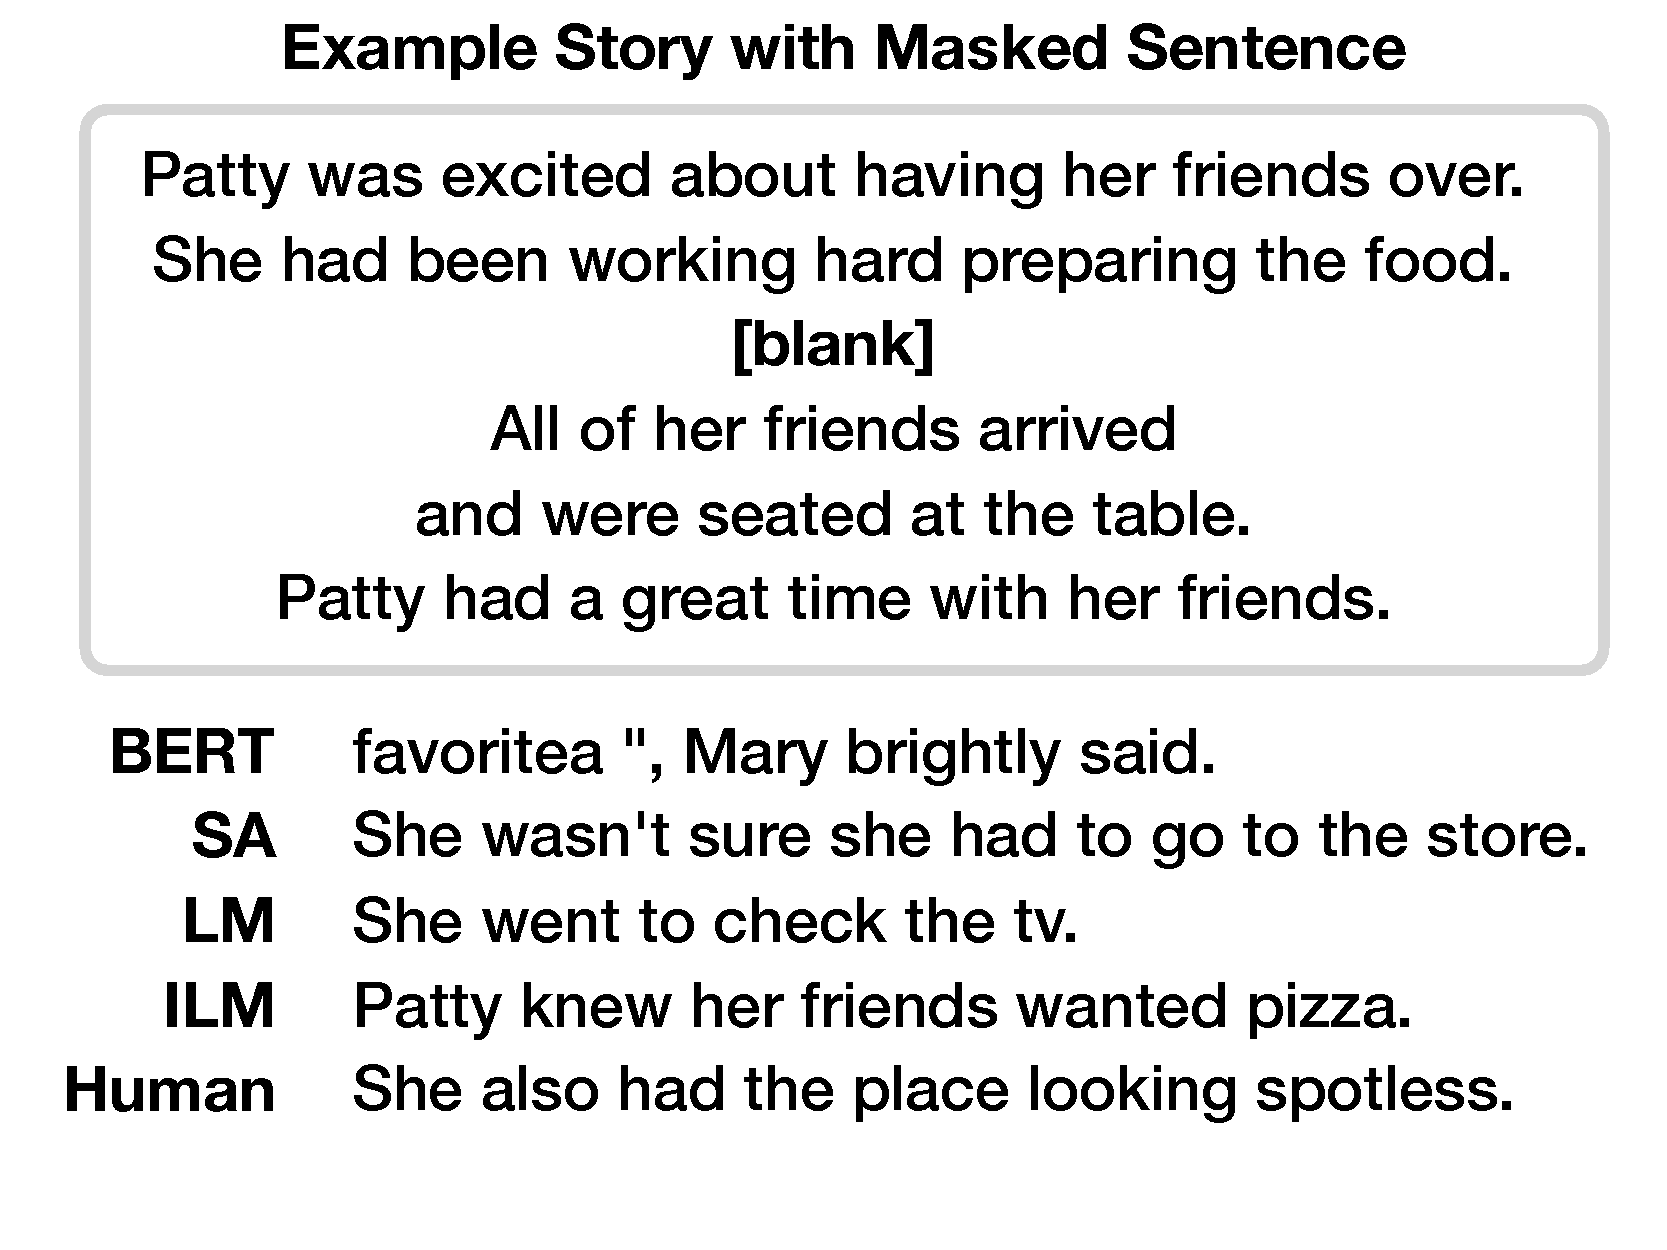
\includegraphics[width=1\linewidth]{figures/ilm_figure3_final.pdf}
    \vspace{-1cm}
    \caption{Example of a short story in our \stories{} dataset with its third sentence masked, and sentences infilled by different models. The sentences generated by BERT and SA models are off-topic, the sentence generated by LM model is irrelevant to the future context, while the ones generated by ILM and Human successfully account for both previous and future context.}
    \label{fig:human_eval_example}
\end{figure}